\documentclass[twoside, 12pt, a4paper]{article}

\usepackage[paper=a4paper,left=25mm,right=25mm,top=25mm,bottom=25mm]{geometry}

%Package for German Language + Sonderzeichen
\usepackage[ngerman]{babel}

%Literaturverzeichnis
\usepackage[square,numbers]{natbib}
%myabbrvnat.bst (in detsch ge�ndert) muss zum Projektordner hinzu
\bibliographystyle{myabbrvnat}

%set space on enumerate 
\usepackage{enumitem}

%Rahmen um Bilder
\usepackage{fbox}

% Package to include Images 
\usepackage{graphicx}
%controll place of image FloatBarrier
\usepackage{placeins}

% smarte referenzierung bei Abbildungen etc. 
\usepackage[hidelinks]{hyperref}
\usepackage[ngerman,noabbrev]{cleveref}
%Label am rand anzeigen
% auskommentieren am Ende um Rote boxen zu entfernen.
%\usepackage{showkeys} 


% include f�r Kopf-/Fu�zeile
\usepackage{fancyhdr}
\pagestyle{fancy}
\fancyhf{}
\renewcommand{\headrulewidth}{0.4pt}
\renewcommand{\footrulewidth}{0.4pt}% default is 0pt

\usepackage[latin1]{inputenc} % erm\"oglich die direkte Eingabe der Umlaute 
\usepackage[T1]{fontenc} % das Trennen der Umlaute
\usepackage{ngerman} % hiermit werden deutsche Bezeichnungen genutzt und 
% die W\"orter werden anhand der neue Rechtschreibung 
% automatisch getrennt.  


\title{ \textbf{ Expose� Masterprojekt:}\\ \vspace{2cm} Acoustic Emission zur Zustands\"uberwachung von menschlichen Gelenken und mechanischen Strukturen}

\author{Florian Mayerle \& \\
	Tim Dedekind \\
	Technische Hoschschule Ulm \\
	Fakult\"at Mechatronik und Medizintechnik\\
	Albert-Einstein-Allee 55\\
	89081 Ulm  \\
	\and 
	Betreuer: Prof. Dr.-Ing. Michael Kaufeld  \\
	
}

\date{\today}


\begin{document} \selectlanguage{ngerman}
	
	%Keine Abs�tze einger�ckt 
	\setlength\parindent{0pt}
	
	\begin{figure}
		\centering
		
		
\includegraphics[width=6cm,keepaspectratio]{Images/THU}
	\end{figure}
	
	\maketitle
	
	\newpage
	\fancyhf{}
	\fancyhead[RO,LE]{\rightmark}
	\fancyfoot[RO,LE]{\thepage}
	\fancyfoot[LO,RE]{THU, Abstrakt AE, Mayerle \& Dedekind }
	%\begin{abstract}
	%\end{abstract}
	
	\newpage
	\setcounter{page}{1}
	\tableofcontents
	\listoffigures
	\newpage
	
	\section{Einf\"uhrung und Motivation}
	
	% Was is AE ?? 
	
	Mechanische und biologische Strukturen geben bei einer Ver\"anderung, wie z.B. einer Dehnung oder einem Bruch messbare Schallsignale ab. Ebenso ist es m\"oglich durch die Aufnahme der Signale \"uber einen l\"angeren Zeitraum hinweg eine Ver\"anderung der Signalcharakteristik zu erkennen. Grund daf\"ur ist beispielsweise der Verschlei{\ss} der mechanischen Struktur und somit eine Ver\"anderung der Oberfl\"ache.\\     
	
	Im medizinischen Bereich werden h\"aufig mehrere kommerziell verf\"ugbarer nicht-invasive Techniken wie R\"ontgen, Ultraschall und Magnetresonanztomografie (MRT) f\"ur die Grundlage einer Diagnoseerstellung genutzt. Ebenso wird diese Technik herangezogen, um Operateure w\"ahrend eines Eingriffs mit Informationen, wie der Position des Werkzeugs oder des Zustands des Implantats, zu versorgen. Zudem werden minimalinvasive Verfahren wie zum Beispiel die  Arthroskopie durchgef\"uhrt, um einen direkten Einblick in den K\"orper zu erhalten.\\
	Diese Techniken liefern visuelle Daten, die Beispielsweise f\"ur die Beurteilung der inneren Gelenkstruktur herangezogen werden. F\"ur die Aufnahme und Auswertung der Daten bedarf es jedoch einer speziellen Ausbildung sowie einem hohen Erfahrungsgrad f\"ur die Diagnoseerstellung. Zudem liefern diese Techniken meist nur eine statische Informationen \"uber den aktuellen Zustand von K\"orper, Ger\"at oder Implantat. Weiterhin ist zu beachten, dass Punkte wie Zug\"anglichkeit und Behandlungskosten, speziell bei einer MRT-Untersuchung, als nachteilig gewertet werden. Eine kosteng\"unstige nicht-invasive Detektionstechnik welche den K\"orperschall von K\"orper oder Ger\"at analysiert, k\"onnte sowohl f\"ur \"Arzte als auch f\"ur Patienten von gro{\ss}em nutzen sein.\cite{Feng.2016}\\
	
	Schlagw\"orter: acoustic emission (AE), structural health monitoring (SHM), Signalclusterung, Burst-Analyse, Schallemission, K\"orperschall-Analyse, Vibroarthographie (VAG), VAG-Signale, joint acoustic emissions (JAEs), joint sounds.   
	
	

	
	\section{Einsatzm\"oglichkeiten von Acoustic Emission Testing}
	
	Das Acoustic Emission Testing (AT) wird in der industriellen Awendung in der Prozess\"uberwachung und ebenso zur  Zustands\"uberwachung eingesetzt.\\
	%Unterscheidung von Prozess und Zustand, oftmals flie�end deswegen genaue definition suchen!!!!. 
	In der Prozess\"uberwachung kann das AT dazu eingesetzt werden, um w\"ahrend eins Fertigungsverfahrens den Zustand des Halbzeugs oder des Werkzeugs zu \"uberwachen. So nutzt die Firma Brankamp die akustischen Signale w\"ahrend eines Stempelvorgangs von Metallblechen, um Stempelbr\"uche oder Matritzenrisse zu detektieren\cite{Brankamp_prospekt}. Ebenso kann das Messprinzip angewendet werden, um w\"ahrend einer zerspanenden Fr\"as- und Drehbearbeitung Abnutzung, Rissbildung und Abplatzung am Werkzeug zu erkennen \cite{DGZfP-Kompendium}.\\
	Das AT wird ebenso zur \"Uberwachung von vielerlei Zust\"anden, \"uber einen l\"angeren Einsatzzeitraum hinweg, eingesetzt. In der Bauindustrie wird \"uber die Ver\"anderung der akustischen Emission eines Bauwerks das Risswachstum in Br\"ucken und Staud\"amme \"uberwacht. Ebenso k\"onnen Leckagen und Gasverluste an Ventilen \"uber akustische Emission nachgewiesen werden. \cite{DGZfP-Kompendium} Diese Art der Zustands\"uberwachung wird auch als Structural Health Monitoring (SHM) bezeichnet.\\
	Von diesen industriellen Anwendungen werden im n\"achsten Abschnitt abgeleitete, medizinische Anwendungen, welche den aktuellen Stand der Technik repr\"asentieren, aufgef\"uhrt.  

	\subsection{Angewandte akustische Prozess\"uberwachung in der Medizin} \label{sec:Angewandte Technik}
	
	In der heutigen Medizintechnikbranche gibt es einigen technische Entwicklungen, die das Prinzip der Analyse von akustischen Emissionen nutzen, f\"ur die aktuell Patente oder sogar bereits realisierte Ger\"ate mit g\"ultiger Marktzulassung existieren. In dem Exposee \grqq
	\href{https://www.innowi.de/de/unsere_patente/details/intelli-drill---knochenbohrer-un388}{Intelli-Drill - Bohren und Messen in einem Schritt}\grqq{} wird das Konzept einer medizinischen Bohrmaschine vorgestellt, welche mithilfe einer K\"orperschallmessung die Bohrtiefe ermittelt. Aus der zugeh\"origen Patentschrift geht hervor, dass die L\"ange des Bohrkanals mithilfe von drei Sensoren (Axialkraft-,Bohreindringtiefen- und K\"orperschallmessung) und einem integrierten Computer errechnet wird.~\cite{Axel.26.08.2011} \cref{img:Intellidrill} zeigt das beim Bohren entstehende akustische Profil, worin die Struktur des zerspanten Knochens, \"uber die unterscheide in Amplitude und Frequenz, zu deuten ist. 
	
	\begin{figure}[!htbp]
		\centering
		\setlength{\fboxsep}{0.5pt}
		\setlength{\fboxrule}{0.5pt}
		\fbox {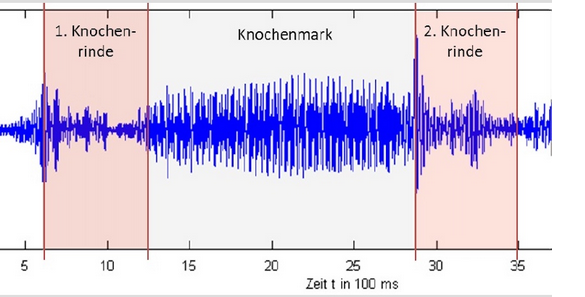
\includegraphics[width=10cm,keepaspectratio]{Images/Intellidrill.PNG}}
		\caption[Intellidrill]{Intellidrill - Bohren und messen in einem Schritt (entnommen aus \cite{UniBremen.21.04.2020})}
		\label{img:Intellidrill}
	\end{figure}
	\FloatBarrier
	
	
	Ein \"ahnliches, schon auf dem Markt erh\"altliches, Produkt \glqq SMARTdrill6.0\grqq{} wurde von der Smart Medical Devices INC. entwickelt. Dieses Bohrger\"at liefert neben der Tiefenkontrolle und -messung auch ein Performancefeedback und sendet die Daten \"uber eine drahtlose Kommunikation an ein Tablet, welches die problemlose \"Uberwachung oder Justierung der Bohr-Parameter erm\"oglicht.~\cite{SMARTdrill.2020} 
	
	\begin{figure}[!htbp]
		\centering
		\setlength{\fboxsep}{0.5pt}
		\setlength{\fboxrule}{0.5pt}
		\fbox {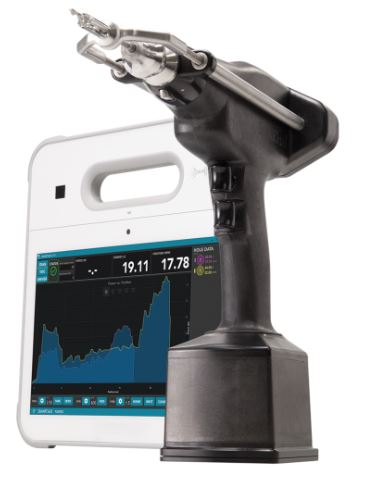
\includegraphics[width=4cm,keepaspectratio]{Images/Smartdrill.JPG}}
		\caption[SMARTdrill6.0]{SMARTdrill6.0 - Intelligenter Bohrer mit \"uberwachungscomputer (entnommen aus \cite{SMARTdrill.2020})}
		\label{img:SMARTdrill.2020}
	\end{figure}
	\FloatBarrier       
	
	Ebenso hat die Firma McGinley Orthopaedic Innovations eine Freigabe von der FDA f\"ur das entwickelte \glqq IntelliSense\grqq{}  System bekommen. Dabei handelt es sich um ein, mit dem \glqq SMARTdrill6.0\grqq{} vergleichbares, Werkzeug zum Bohren von Knochen.\\
	\\
	Die vorangegangenen technischen Beispiele zeigen, dass die Anwendung von AE in medizintechnischen Ger\"aten ein hoch innovatives Feld ist, in welchem immer noch viel geforscht wird um Prozesse durch gezielte \"Uberwachung noch effektiver ausf\"uhren zu k\"onnen. 


	\subsection{Zustands\"uberwachung in der Medizin}
	
	In der Medizin wird die Schallemissionsanalyse nicht nur zur Prozess\"uberwachung, sondern auch zur Zustands\"uberwachung eines menschlichen Bewegungsapparats genutzt. Die praktische Anwendung wird in einem von der Firma Bonedias 2019 vorgestelltem Produkt (Abbildung \ref{img:Bonedias}) deutlich. \"uber die Messung der Schallemission w\"ahren einer definierten Bewegung, wie zum Beispiel einer Kniebeuge, erkennt dieses Ger\"at ein Schallmuster, welches von dem eines gesunden Gelenks abweicht. Im Abgleich mit MRT-Aufnahmen wird eine \"Ubereinstimmung der Befunde beider Technologien von 95\% erreicht, womit die Funktionalit\"at dieses Ger\"ats bewiesen wird. Bei den 5\% falsch positiv klassifizierten Befunden wird sogar davon ausgegangen, dass die Messung der Schallemission sensitiver als die herk\"ommliche MRT-Diagnostik ist und die Daten genutzt werden k\"onnen, um vorbeugende Therapien zu erm\"oglichen.~\cite{Oppermann.2019}  	
	
	\begin{figure}[!htt]
		\centering
		\setlength{\fboxsep}{0.5pt}
		\setlength{\fboxrule}{0.5pt}
		\fbox {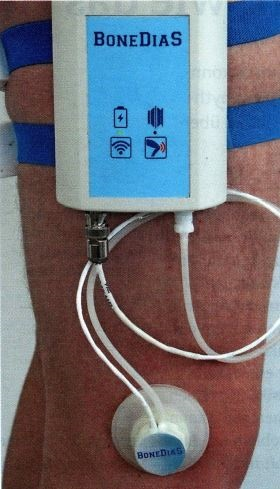
\includegraphics[width=4cm,keepaspectratio]{Images/Bonedias.JPG}}
		\caption[Bonedias]{Bonedias - Aufnahmeger\"at mit Tonabnehmer der Firma Bonedias aus Greifenstein (entnommen aus \cite{Oppermann.2019})}
		\label{img:Bonedias}
	\end{figure}
	\FloatBarrier
	
	
	Die Idee K\"orperschall oder bioakustische Signale zu nutzen, um den Zustand von Gelenken im menschlichen K\"orper zu \"uberwachen wurde bereits 1987 von Gerald F. McCoy et al. erforscht. Dieser untersuchte normale, sowohl als auch symptomatische Gelenke und konnte daraufhin mehrere symptomatische Signaltypen von drei normalen Signaltypen unterscheiden. Er erkannte, das AE-Testing ein enormes Potenzial als diagnostisches Hilfsmittel bei Erkrankungen des Knies besitzt und baute auf die fortschreitende Entwicklung der Computertechnik, um akkuratere Diagnosetools realisieren zu k\"onnen.~\cite{McCoy.1987}
	
	
	
 	\newpage
	
	
	\subsection{Auswerten und Clustern von Daten}
	
	Das aufgenommene akustische Signal alleine liefern noch keine Information \"uber einen Zustand oder einen Prozess am menschlichen K\"orper. Dazu m\"ussen die Signale erst nachbearbeitet und analysiert werden. Diese Informationen liefert nicht nur die Amplitude, sondern vor allem das Frequenz und Leistungsspektrum. Zur Untersuchung kann das Signal nun \grqq{}h\"andisch\grqq{} ausgewertet werden, in dem man eine Fourier- oder Wavelet Transformation durchf\"uhrt und Unterschiede im Frequenzspektrum der Signale erkennt. Eine andere M\"oglichkeit bietet die Verwendung eines Algorithmus zur automatischen Datenclusterung.\\
	Als Cluster wird eine Sammlung von einander \"ahnlichen Objekten bezeichnet. Au�erhalb des Cluster befinden sich alle un\"ahnlichen Objekte. Die Bewertung der \"Ahnlichkeit erfolgt mit mathematischen Funktionen welche mithilfe verschiedenen Algorithmen berechnet werden. Das Ergebnis der Clusterung l\"asst sich anschlie�end automatisch oder manuell bewerten woraufhin der Clusterprozess auf Basis dieser Bewertung spezifisch angepasst werden kann. Zweck der  Datenclusterung ist, eine Datenmengen in m\"oglichst unterschiedliche und aussagekr\"aftige Cluster zu  unterteilen. So zum Beispiel k\"onnten Signalbereiche der Bohrprozesse am Knochen den verschiedenen Knochenstrukturen oder Ereignissen (Bruch der Schneide, Durchbruch des Bohrkanals) zugeordnet werden. Die Cluster k\"onnen dann einzeln untersucht, oder mehrere Cluster miteinander verglichen werden. Dies vereinfacht die Analyse von sehr gro�en Datenmengen. Durch Clusteranalysen ist es auch m\"oglich nat\"urliche Gruppen in den analysierten Daten zu finden. Dadurch l\"asst sich Wissen \"uber die nat\"urliche Struktur und die spezifischen Eigenschaften der Daten gewinnen. \cite{CanOnder.15.01.2004},~\cite{PhilipPlohn.2014}~ Die in den sp\"ateren Versuchen gesammelten Daten sollen mithilfe von Clusteranalysen untersucht werden. Zur Clusterung wird das Signal in Bursts, also k\"urzere, zeitlich begrenzte Signale, unterteilt, die dann nach Merkmalen wie Peak Frequenz oder Burstanzahl pro Zeit geclustert werden k\"onnen. 
	
	%kontinuierlichen und impulsf\"ormigen Signalen, den so genannten Bursts
	
	
	\section{Zielsetzung des Masterprojekts}
	
	
	Hauptziel des Masterprojekts ist es, die in Abbildung \ref{img:SensorToolchain} dargestellte Sensor-Toolchain zur Erfassung und Clusterung von akustischen Signalen in der industriellen Anwendung drauf hin zu \"uberpr\"ufen, ob diese ebenso f\"ur die Anwendung im medizinischen Bereich geeignet ist. Die Toolchain besteht aus der iNDTact-Messsoftware f\"ur die Datenaufnahme und Datenauswertung, einem DAQ-Tool (Messchassi NI cDAQ-9188 und Analogwandler NI 9223 von National Instruments), einer Verst\"arkerbox und dem eigentlichen iNDTact iMPact XS piezoelektrischen Sensor.
	  
	
		\begin{figure}[!htbp]
		\centering
		\setlength{\fboxsep}{0.5pt}
		\setlength{\fboxrule}{0.5pt}
		\fbox {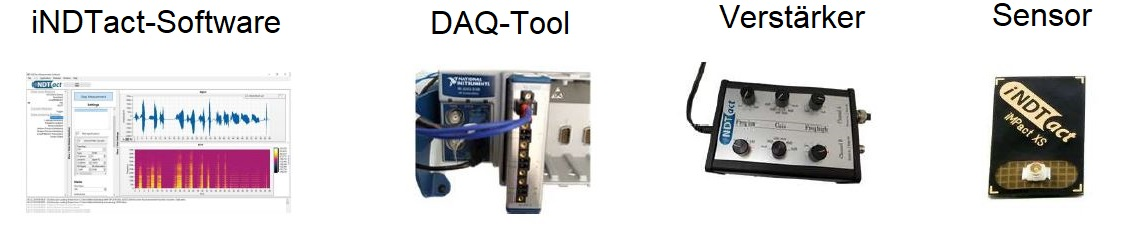
\includegraphics[width=17cm,keepaspectratio]{Images/SensorToolchain.JPG}}
		\caption[SensorToolchain]{SensorToolchain - Software, Daq-Tool, Verst\"arker-Box und Sensor}
		\label{img:SensorToolchain}
		\end{figure}
		\FloatBarrier   
	
	Idee oder Hypothese ist, dass diese Toolchain sich m\"oglicherweise sehr gut (vergleichbar) oder gegebenenfalls besser, als bisher eingesetzte Systeme, zum AE-Testing in der Medizintechnik eignet. Diese Hypothese basiert auf folgenden Aspekten: 
	
	\begin{itemize}
		\item{\textbf{Multifunktionale Mess- und Analysesoftware:} Mit dieser Software ist, in Kombination mit dem Analogwandler, ein Abtasten des Sensors mit einer Rate von bis zu 1MHz m\"oglich. Dadurch k\"onnen Signale bis hin zu einem Frequenzbereich von 0.5MHz analysiert werden. zudem bietet die Software umfangreiche Analyse und Cluster M\"oglichkeiten.}
		\item{\textbf{Pr\"azise Verst\"arker-Box:} Mit der Verst\"arker-Box k\"onnen sehr schwache Signale, mit bis zu 60dB, hoch verst\"arkt werden, dies erm\"oglicht die Aufnahme von minimalen akustischen Emissionen am K\"orper bei der Bewegung von Gelenken. Ebenso kann \"uber das einstellen einer geringen Verst\"arkung von -40dB sehr hohe akusstische Emissionen erfasst werden, welche zum beispiellos beim Bohren von Knochen entstehen.}	
	\end{itemize} 

	Diese Hypothese wird mit Hilfe einer umfangreichen Literaturrecherche \"uberpr\"uft. Der Fokus dabei liegt darin den Stand der Technik, im Hinblick auf verwendete Sensoren, erfasster Frequenzbereich, Verarbeitung und Filterung der Signale sowie verwendete Analysetools und Quantifizierungsparameter, zu erfassen. Da der Einsatz von AE-Testing im medizinischen Bereich ein breites Feld ist, fokussieren wir uns bei der Literaturrecherche auf das Gebiet der Prozess\"uberwachung (Bohren, Fr\"asen, Schaben von Knochen oder Z\"ahnen). Es soll lediglich ein \"Uberblick auf Themen aus der Zustands\"uberwachung gegeben werden \\    
	Im praktischen Teil soll, \"uber die im n\"achsten Kapitel beschriebenen Tests, die Einsatzm\"oglichkeit der Toolchain im medizinischen Bereich erprobt werden. Der Fokus dabei liegt ebenfalls auf dem Gebiet der Prozess\"uberwachung . 
	Mit dieser Arbeit soll ein Basiswissen geschafft werden und m\"ogliche Forschungsziele er\"ortert werden um dann im darauf Folgenden Projekt gezielt an einer Fragestellung arbeiten zu k\"onnen. Folgend die Ziele noch einmal in wenigen Worten zusammengefasst.
	
	\begin{itemize}
		\item {Aufbau von Wissenshintergrund und technischem Rahmen f\"ur	weitere Forschung.}
		\item {F\"ur welche medizinischen Anwendungen kann die Toolchain verwendet werden?} 
		\item {Gibt es Vorteile im Vergleich der Toolchain zum Stand der Technik?} 
		\item {Identifizieren von m\"oglichen Forschungsschwerpunkten basierend auf offenen Fragen nach auf den Stand der Technik.}
	\end{itemize} 
	
	 
	
	
	
	\section{Initiale Arbeitsschritte}
	
Die Initialen Arbeitsschritte beinhalten eine umfangreiche Literaturrecherche zum Thema AE-Testing in der medizinischen Prozess\"uberwachung, sowie erste praktische Tests. \\


Das Ziel der Tests ist es, zu untersuchen, ob sich der IndTact Impact XS Sensor zur Benutzung im medizinischen Process Monitoring eignet. Dazu wird untersucht, ob sich beim Bohren in Z\"ahnen und Knochen Unterschiede zwischen verschiedenen Knochen- und Zahnschichten erkennen lassen. Anschlie�end erfolgt ein Test, der die verschiedene Applikationsm\"oglichkeiten untersucht, um festzustellen, ob es hier Unterschiede zwischen den aufgenommenen Signalen gibt. Der vierte Test liefert noch einen Ausblick \"uber eine m\"ogliche Nutzung des Sensors im medizinischen Condition Monitoring. Hier wird mit ersten Tests untersucht, ob sich generell \"uber Acoustic Emission Messungen mit dem IndTact Sensor ein Signal vom menschlichen K\"orper aufnehmen l\"asst, welches sich als sogenannter Biomarker eignet.  

\begin{enumerate}
	\item{\textbf{Test:} Durchbohren von Knochen zur Clusterung des Knochenmaterials  }
	\item{\textbf{Test:} Fr\"asen von Z\"ahnen zur Clusterung des Zahnmaterials}
	\item{\textbf{Test:} Selbstversuch, Aufnahme von Biosignalen am Knie}
\end{enumerate}


\subsection{Schwerpunkte Literaturrecherche:}

Die Literaturrecherche wird auf den Bereich der Prozess\"uberwachung in der Medizintechnik beschr\"ankt. Folgende Informationen sind von Interesse: 

\begin{itemize}
	\item{Prozessparameter (Drehzahl, Druck, .... )}
	\item{Quantifizierungsparameter (RMSE,Mean, ...)}
	\item{Signalverarbeitung und Filter }
	\item{Frequenzbereich } 
	\item{Sensortypen (MEMS, piezoelektrisch, Kondensator, ...) }
	\item{Signalauswertungstools und Algorithmen}
\end{itemize}

\subsection{Beschreibung von Test 1, (Bohren von Knochen)}

Im ersten Versuch sollen Bohrungen an tierischen Knochen durchgef\"uhrt werden. In Abbildung 1 werden die unterschiedlichen Knochenschichten (Spongiosa und Kortikalis) dargestellt. Die beim Zerspanen der verschiedenen Schichten entstehenden unterschiedlichen akustischen Emissionen sollen dabei aufgenommen und geclustert werden. Ziel ist es f\"ur die verschiedenen Strukturen und Knochendichten akustische Muster zu erkennen um bei der Bearbeitung von Knochen R\"uckschl\"usse auf Bohrtiefe und Materialzusammensetzung schlie�en zu k\"onnen. Ebenso soll untersucht werden, wie sich das Signal ver\"andert, wenn der Knochenbohrer aus der Bohrung austritt oder w\"ahrend des Bohrens auf einen Hohlraum trifft. Der akustische Sensor wird, anders als in der Abbildung 1 skizziert in direktem Kontakt mit dem Knochen appliziert. Um den Einfluss der Anpresskraft des Bohrwerkzeugs auf das akustische Signal zu ermitteln wird in die Bearbeitungsplattform eine Kraftmessplatte integriert, deren aufgenommene Daten sp\"ater mit den Acoustic Emission Daten abgeglichen werden.



	
	
		\begin{figure}[!htbp]
		\centering
		\setlength{\fboxsep}{0.5pt}
		\setlength{\fboxrule}{0.5pt}
		\fbox {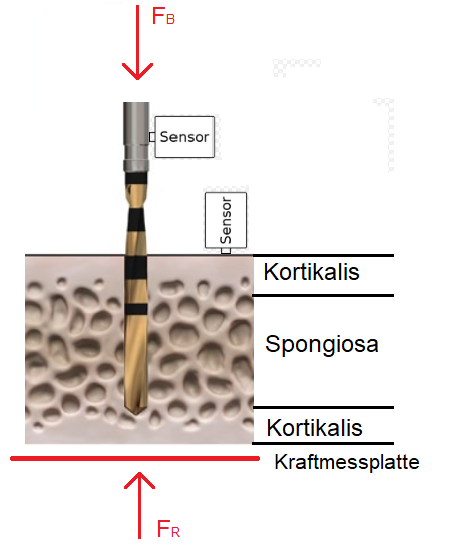
\includegraphics[width=6cm,keepaspectratio]{Images/KnochenBohren.png}}
		\caption[Knochen Bohren]{Knochen Bohren - Testaufbau (entnommen aus \cite[S. 6]{Dentsply.21.04.2020})}
		\label{img:Knochen Bohren}
	\end{figure}
	\FloatBarrier
	
\subsection{Beschreibung von Test 2 (Fr\"asen von Z\"ahnen)}	

Im zweiten Versuch sollen Fr\"asungen an menschlichen Z\"ahnen durchgef\"uhrt werden. Die beim Zerspanen der verschiedenen Schichten entstehenden unterschiedlichen akustischen Emissionen sollen dabei aufgenommen und geclustert werden. Ziel ist es f\"ur die verschiedenen Strukturen akustische Muster zu erkennen, um bei der Bearbeitung von Z\"ahnen auf die unterschiedliche Materialzusammensetzung schlie�en zu k\"onnen. Ebenso soll untersucht werden, wie sich das Signal ver\"andert, wenn der Fr\"aser von einer Zahnsubstanz auf die andere wechselt.\\
Der akustische Sensor wird entweder in direktem Kontakt mit dem Zahn oder mit indirektem Kontakt zum Zahn an dem Geh\"ause des Bearbeitungswerkzeugs appliziert. Um den Einfluss der Anpresskraft des Fr\"aswerkzeugs auf das akustische Signal zu ermitteln wird in die Bearbeitungsplattform eine Kraftmessplatte integriert. Die Daten der Kraftmessplatte werden zur Versuchsauswertung mit den Acoustic Emission Daten verglichen, um den St\"orfaktor der Anpresskraft zu ber\"ucksichtigen.



\subsection{Beschreibung von Test 3, Schallemission am Kniegelenk}	


Im Selbstversuch soll zun\"achst \"uberpr\"uft werden, ob und in welcher Qualit\"at mit dem vorhandenen iNDTact Messequipment akustische Signale in verschiedenen Bewegungsszenarien vom menschlichen Bewegungsapparat erfasst werden k\"onnen. Ebenso soll untersucht werden, ob das aufgenommen Signal \"uber eine Clusterung der spezifischen Bewegung zugeordnet werden kann. Weiterhin k\"onnten, bekannte defekte am Bewegungsapparat genutzt werden, um Beispielsweise zu untersuchen ob sich die akustische Emission, eines defekten Gelenks (Knie/Finger) im Vergleich zum gesunden gegen\"uberliegenden Gelenk, unterscheidet.




	
	\begin{flushleft}
		%literaturverzeichnis Datei einbinden
		\bibliography{bibliography}
	\end{flushleft}
	
\end{document}
